\documentclass[paper=a4]{ctexart} % A4 paper and 11pt font size
\usepackage{fontspec,caption, xeCJK,amsmath,tocvsec2,extarrows, chngpage, adjustbox, clrscode}
\usepackage{listings}
\usepackage[T1]{fontenc} % Use 8-bit encoding that has 256 glyphs
\usepackage[english]{babel} % English language/hyphenation
\usepackage{amsmath,amsfonts,amsthm,amssymb, enumerate} % Math packages
\usepackage{framed,floatflt}   
\usepackage{graphics}
\usepackage{graphicx}
\usepackage{picins}
\usepackage{lipsum} % Used for inserting dummy 'Lorem ipsum' text into the template

\usepackage{sectsty} % Allows customizing section commands
% \allsectionsfont{\centering \normalfont\scshape} % Make all sections centered, the default font and small caps
\usepackage{wrapfig}
\usepackage{fancyhdr} % Custom headers and footers
\pagestyle{fancyplain} % Makes all pages in the document conform to the custom headers and footers
\fancyhead{} % No page header - if you want one, create it in the same way as the footers below
\fancyfoot[L]{} % Empty left footer
\fancyfoot[C]{} % Empty center footer
\fancyfoot[R]{\thepage} % Page numbering for right footer
\renewcommand{\headrulewidth}{0pt} % Remove header underlines
\renewcommand{\footrulewidth}{0pt} % Remove footer underlines
\setlength{\headheight}{13.6pt} % Customize the height of the header

\numberwithin{equation}{section} % Number equations within sections (i.e. 1.1, 1.2, 2.1, 2.2 instead of 1, 2, 3, 4)
\numberwithin{figure}{section} % Number figures within sections (i.e. 1.1, 1.2, 2.1, 2.2 instead of 1, 2, 3, 4)
\numberwithin{table}{section} % Number tables within sections (i.e. 1.1, 1.2, 2.1, 2.2 instead of 1, 2, 3, 4)

\lstset{
        keywordstyle=\color{blue}, %设置关键字颜色
        commentstyle=\color[cmyk]{1,0,1,0}, %设置注释颜色
        frame=single, %设置边框格式
        escapeinside=``, %逃逸字符(1左面的键),用于显示中文
        breaklines, %自动折行
        extendedchars=false, %解决代码跨页时,章节标题,页眉等汉字不显示的问题
        xleftmargin=2em,xrightmargin=2em, aboveskip=1em, %设置边距
        tabsize=4, %设置tab空格数
        showspaces=false %不显示空格
       }

\setlength\parindent{0pt} % Removes all indentation from paragraphs - comment this line for an assignment with lots of text

% ----------------------------------------------------------------------------------------
% TITLE SECTION
% ----------------------------------------------------------------------------------------
\newcommand{\get}{\Longrightarrow}
\newcommand{\Sum}{\displaystyle \sum}
\newcommand{\p}[1]{\subsection{Problem~{#1}}}
\newcommand{\horrule}[1]{\rule{\linewidth}{#1}} % Create horizontal rule command with 1 argument of height
\title{
  \normalfont \normalsize 
  \textsc{\\~\\~\\~\\~\\~\\University of Science and Technology of China} \\ [25pt] % Your university, school and/or department name(s)
  \horrule{0.5pt} \\[0.4cm] % Thin top horizontal rule
  \huge 基于Inferno的集群与并行计算框架 \\ % The assignment title
  \horrule{2pt} \\[0.5cm] % Thick bottom horizontal rule
}

\usepackage{enumitem}

\setcounter{footnote}{-1} %第一个footnote不显示标号


\newcounter{newlist} %自定义新计数器
\newenvironment{denselist}[1][可改变的列表题目]{%%%%%定义新环境
\begin{list}{\textbf{\hei #1} \arabic{newlist}:} %%标签格式
{
\usecounter{newlist}
\setlength{\labelwidth}{22pt} %标签盒子宽度
\setlength{\labelsep}{0cm} %标签与列表文本距离
\setlength{\leftmargin}{0cm} %左右边界
\setlength{\rightmargin}{0cm}
\setlength{\parsep}{0ex} %段落间距
\setlength{\itemsep}{0ex} %标签间距
\setlength{\itemindent}{44pt} %标签缩进量
\setlength{\listparindent}{22pt} %段落缩进量
}}
{\end{list}}%%%%%

\newcommand{\n}{\\\indent}
\author{\Large{阮震元~~~~解宇飞~~~~杨智~~~~刘旭彤}\footnote{阮震元~:~PB13011009,联系方式rzyrzyrzy2014@gmail.com,科技实验楼1406系统设计室}
\setcounter{footnote}{-1}
\footnote{解宇飞~:~PB13011001~~~~杨智~:~PB13011079~~~~刘旭彤~:~PB13011072}
} % Your name
\date{} % Today's date or a custom date

\begin{document}

\maketitle % Print the title

% 目录
% 可以直接编辑toc文件来更改目录
\clearpage
\setcounter{section}{0}
\setcounter{subsection}{0}
\setcounter{subsubsection}{0}
\tableofcontents
\clearpage
% 改变层次目录来达到section和subsection默认不编号(需要tocvsec2包)

\section{调研报告}

\subsection{项目背景及实践意义}

\subsubsection{项目的背景}
如今人类各个学科繁多、涉及面广、分类细致,而且不同学科之间又有交叉.而如今很多的学科都需要进行大量的计算,如天文学研究组织需要计算机来分析太空脉冲,星位移动;生物学家需要计算机来模拟蛋白质的折叠过程;药物学家需要计算机来研制克服爱滋病或非典的药物;数学家需要计算机来计算最大的质数和圆周率的更精确值;经济学家也要用计算机分析计算在几万种因素考虑下某个企业/城市/国家的发展方向从而宏观调控.由此可见,未来科学的发展离不开计算.在很多时候,为了进行研究而特地去购买一台专用的超级计算机往往是不现实的.而分布式计算,因为其高效而便宜的特点,越来越受社会的关注.\n
为了说明目前国内分布式计算的现状,我们参考了BOINC平台的一些数据. \n
BOINC,也即伯克利开放式网络计算平台(Berkeley Open Infrastructure for Network Computing),是目前主流的分布式计算平台之一.作为一个高性能的分布式计算平台,截止至2015年1月16日,BOINC在全球有235,980位活跃的参与者以及692,208台活跃的主机,提供约9.871 petaFLOPS的运算能力(天河二号超级计算机运算速度约为33.86 petaFLOPS).\n
以生命科学为例,下面是一些运行在BOINC平台下的项目:
\begin{enumerate}
\item Discovering Dengue Drugs : 针对登革热、丙型肝炎、西尼罗河病毒和黄热病病毒发现有前途的药物先导化合物
\item Genome Comparison : 染色体对比研究
\item Help Conquer Cancer : 帮助科学家征服癌症
\item Help Defeat Cancer : 帮助科学家对抗癌症
\item Human Proteome Folding : 人类蛋白质折叠研究 
\item Human Proteome Folding 2 : 人类蛋白质折叠第2阶段研究
\item Help Cure Muscular Dystrophy : 针对肌肉营养失调和其他神经肌肉型疾病的研究
\item Nutritious Rice for the World : 针对水稻预测蛋白质结构的研究,以提高水稻产量
\end{enumerate}

\subsubsection{分布式操作系统}
分布式操作系统(Distributed operating system)是在互不依赖的、联网的、相互通信的、物理上分离的多个节点上的软件.每个独立的节点包含一部分整体的操作系统上软件的子集.每个子集都可分为两个不同的部分.第一部分是一个通用的微内核,这个内核直接控制节点上的硬件资源.第二部分是一些高层次的系统管理程序,用来协调节点上独立的和相互协作的活动.这两个部分可以把多节点上的资源和处理能力整合成一个高效并且稳定的系统.因此,尽管这个系统上包含了很多的节点,但是在用户和应用程序看来,这就像是一个节点一样.

\begin{figure}[htbp]
\centering
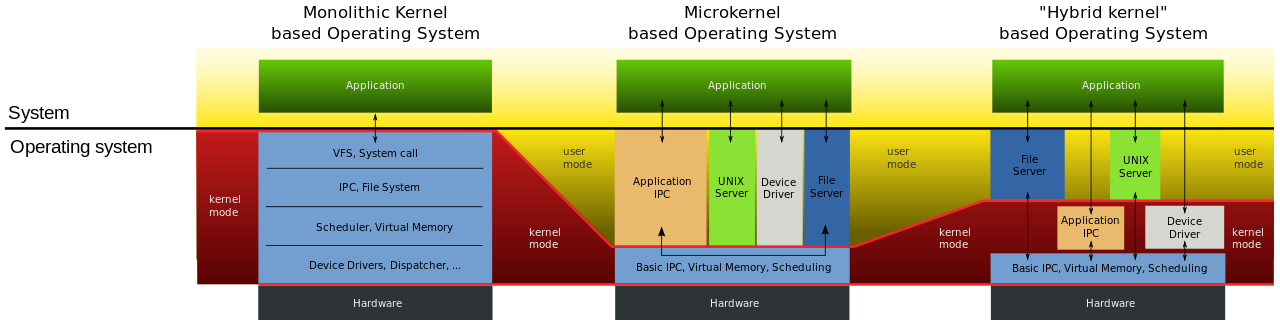
\includegraphics[width=4.8in,height=1.5in]{pic/1.png}
\caption{分布式操作系统的架构}
\end{figure}


\subsubsection{分布式计算}
分布式计算是指把一个需要拥有强大计算能力的超级计算机才能解决的问题分割成小部分,通过分配给许多计算机单独进行计算,整合汇总的局部结果最终得到最终结果,达到虚拟计算机解决大型问题的效果.\n
如今很多领域都采用了这种用分布式系统搭建集群并实现并行计算的方式来进行复杂问题的处理.例如蛋白质疾病分布式计算项目.这个项目主要研究蛋白质折叠、误折、聚合及由此过程引起的一些相关疾病的分布式计算工程.该项目使用联网式的计算方式和大量的分布式计算能力来模拟蛋白质折叠的过程,该过程需要尽量大量、复杂的计算.通过利用世界各地闲散的计算资源,我们可以加快该项目的进程.

\subsubsection{分布式系统实现并行计算的主要问题}

\begin{enumerate}
\item 分布式的数据和文件管理 : 在搭建起大规模的集群时,必须考虑数据分布存储的管理以及访问问题.唯有解决了这个问题,才能够保证并行计算结果的正确性以及并行计算的性能.
\item 数据访问和通信控制 : 在分布式存储访问结构的系统中,数据在不同节点间传输,由于不同节点的运算速度不一致,此外,还有数据访问/通信的时间延迟等问题的存在,所以必须考虑数据和计算同步问题.
\item 可靠性 : 在某些情况下,如网络连接失败,节点可能会失效,进而导致数据丢失、程序终止、乃至系统崩溃等问题的发生.因此,为保证可靠性,必须考虑数据丢失后的恢复以及程序和系统崩溃后的恢复.
\item 网络互联结构的选择 : 不同的节点链接的结构会对系统整体的可靠性以及整体的运算速度产生重大影响.因此,必须根据实际需要、实际情况,权衡各个因素,选择最合适的节点链接结构,如主从非对称结构、环形结构、互联网络结构等.
\item 并行计算的任务划分和算法设计 : 并行计算需要将一个大的计算任务分解成数量合适的小任务,把这些小任务分配给不同的节点或者处理器进行处理,最终收集各个节点/处理器返回的局部结果,并最终整合为一个大的结果.其中并行计算的形式主要有算法分解和数据划分.在分解和划分时,要充分利用各节点、处理器的性能,从而提高运算速度.
\item 并行计算程序设计框架的设计以及实现 : 为了保证并行计算的正确性以及高效性,程序员需要考虑各种各样繁琐的技术细节:数据的存储管理、计算任务的划分、任务的调度执行、数据和计算的同步、结果的收集、节点实效后的恢复等.如何使这些底层细节透明化、自动实现并行计算,是一个很重要的问题.
\item 如何度量并行计算的性能 : 度量并行计算性能的指标是并行计算技术的核心.
唯有有了一个确定的指标,才能设计出合适的算法以及实现方式.
\end{enumerate}

\subsubsection{Inferno操作系统}

根据调研,我们最终决定使用开源的分布式操作系统Inferno来实现分布式计算.\n
Inferno是一个由贝尔实验室研究发明的开源的分布式操作系统,现在由Vita Nuova继续发展和维护.它基于贝尔实验室plan9的经验和该实验室对os、语言、实时编译器、网络、移植等相关方面的研究.\n
\begin{figure}[htbp]
\centering
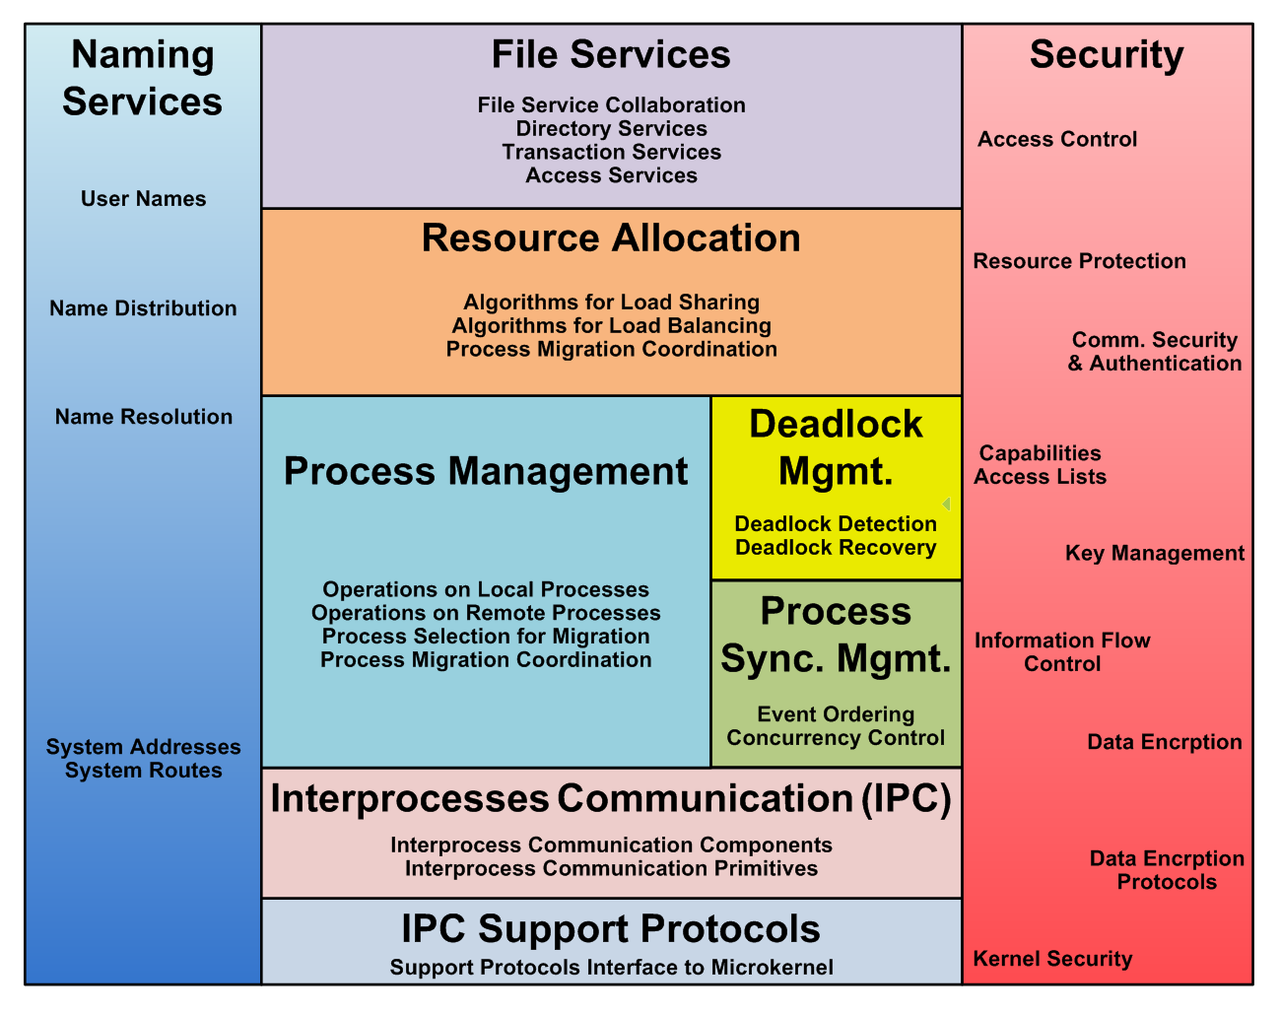
\includegraphics[width=4.8in,height=3.5in]{pic/2.png}
\caption{Inferno的架构}
\end{figure}
该系统定义了一个名为Dis的虚拟机,Dis可在不同的机器上实现.\n
Inferno也提供了一个虚拟的、提供相同借口的操作系统,这个操作系统可以让用户在硬件上直接运行Inferno或者在其它系统中以应用程序的方式运行Inferno. \n
为了让应用程序以统一的方式进行文件操作,如打开、关闭、读写,Inferno采用了一种名为Styx的通信协议.\n
作为一个分布式操作系统,Inferno的设计基于以下三个基本原则:
\begin{itemize}
\item Resources as files: 所有的资源都以分层次的文件的形式存在于文件系统中.
\item Namespaces: 在应用程序看来,网络是一个单一的、条理清楚的namespace(命名空间).虽然这个namespace看起来像是一个分层次的文件系统,但实际上,它表示的是分散的资源.
\item Standard communication: 通过一个名为Styx的协议来访问所有本地和远程的资源.
\end{itemize}

\subsection{小组成员相关背景}
\begin{center}
  \bf{阮震元}
\end{center}
\begin{enumerate}
\item 第二届全国RDMA编程挑战赛冠军
\item 现任科大超算曙光队主力队员,7月将代表科大出征国际超算竞赛
\item 高中时获全国信息学联赛一等奖
\item Topcoder SRM DIV 1
\item Coderforces DIV 1
\item 中国最大计算器论坛cnCalc超级版主
 \end{enumerate}
\hspace{0.75cm}
5年编程开发经验,熟悉C,C++,Java,Python,Scala,Pascal,Deiphi等语言,CUDA,OPENMP,MPI等并行技术.有JavaSE,JavaWeb开发经历,Linux运维经验.高中时获信息学联赛一等奖,Topcoder SRM DIV 1,Coderforces DIV 1,有丰富的算法竞赛经历.大二参加全国RDMA编程挑战赛,具体内容是把分布式处理框架Spark\footnote{http://spark.apache.org/}的IO部分从TCP/IP协议移植到RDMA协议,大幅度提高IO吞吐率从而达到加速效果,获冠军.现任科大超算队队员,即将出征今年7月在德国汉堡举行的国际大学生超算竞赛,在队内负责大型分子动力学模拟软件LAMMPS\footnote{http://lammps.sandia.gov/}的优化加速工作.同时在队内担任系统管理员一职,现管理两个超算系统共十余个节点.

\subsection{立项依据}

\subsubsection{项目意义}
本项目的目标是在具有强大可移植性的分布式操作系统Inferno上实现一个通用并行计算框架,使用户在不了解Inferno分布式资源细节的情况下方便地开发并行程序.\n
 目前流行的并行计算框架如:基于消息传递的“裸”并行编程模型MPI:使用Nvdia加速卡的CUDA; 基于同步数据流的MapReduce,Spark,Prlter:基于数据流水线的Dryad/DryadLINQ,SCOPE,基于存储共享的Piccolo,用于图计算的Pregel,Apache等.本项目所实现的基于分布式操作系统Inferno的分布式结构和rstyx网络协议的并行计算框架属于独创性工作.\n
本项目利用Inferno系统方便的分布式资源管理解决了分布式数据存储管理的问题,通过rstys协议解决通信控制问题.\n
相比CUDA而言,我们并不需要特殊的硬件,只需每台节点上装有Inferno.对于OpenMP而言,我们不仅可以和他一样方便使用一条预处理指令即可自动对for,while等实现并行化,还可以直接看到由我们的解释器翻译出来的并行化代码(保证可读性和可扩展性),甚至可以自己再进一步修改优化.相比MPI我们则不需要实现复杂的通信接口,一切都基于Inferno强大的网络协议Styx,Rstyx.相比MapReduce,Spark而言,我们利用Inferno天然的分布式特点,使用脚本即可实现类似于Map,Reduce的函数.

\subsubsection{理论依据}

\paragraph{资源即文件}

所有Inferno的本地和远程资源都被表示为分层文件系统内的一组动态的文件,这些文件可以表示存储设备、进程、服务、网络和网络连接.应用程序可以通过使用标准的文件操作要求来操作相关的文件进而访问每个资源.使用文件为系统中心概念的优点是:
\begin{itemize}
\item 文件系统具有跨多种操作系统的简单和易于理解的界面,文件界面一般有一套定义好的操作,例如打开,读,写.
\item 通过文件系统降低了代码量,并保持Inferno系统简单、可靠和高度轻便的特性.
\item 对众所周知的文件使用惯例命名,便于统一和理解.
\item 便于确定文件的访问权限和文件许可,可以用于确保多级别的安全性.
\end{itemize}
\hspace{0.75cm}文件名和这些文件的动态的内容可以基于每个需求和每个客户端的基础上产生.例如对于一个传感器资源的数据文件在不同的时间读取就会返回不同的输出,或者每次读取都会在新的一行添加一个数据.这种特性是实现并行计算数据共享的基础之一.

\paragraph{命名空间}
 Inferno的第二个关键原理就是可计算的命名空间,通过命名空间每个应用程序会对它需要访问的资源建立一个独一无二的私有视角,所有的资源被表示为文件的层次结构,并且通过标准文件访问操作来访问,一个进程所使用的各种文件和服务都被一个单根分层文件系统组合起来,叫做命名空间.一个名称空间内访问的资源可以位于单个客户端或在整个网络中的多个服务器.\n
    命名空间系统的主要优点是应用程序可以使用的资源完全透明,在应用程序可见的命名空间中挂载的所有动态资源文件,无论是本地的还是远程的,该应用程序都可以方便的访问.例如,一个图形化的调试器通过读取在/prog目录下的动态文件来访问关于目前系统进程的信息,如果用户希望在另一台远程机器上调试,只需将原来那台机器的/prog目录挂入目前这台机器,对于调试器而言,它只是读取在/prog目录中的文件,但并不知道他们来自哪里.

\paragraph{使用标准通信协议来访问资源}
  Inferno使用一个被Inferno内核或应用程序执行的协议来表示或访问资源.因为所有的资源都被表示为文件,包括网络和网络连接,所以需要一个协议来和提供本地与远程资源的通信.这个协议是一个叫9P的文件服务协议(Styx是一个更早的变体).这种方法就为我们利用已知的技术建立添加远程文件系统的分布式系统提供了一个自然的途径.拥有一个标准通信协议还提供了一个关注安全的点,Inferno提供了下面几种安全通信机制:
  \begin{itemize}
  \item 基于证书的用户认证.
  \item 消息加密.
  \end{itemize}

\subsection{目前所调研到的相关工作}

\subsubsection{Inferno相关调研}
对于Inferno系统的调研的目的是利用Inferno系统方便的分布式资源管理以及sytx通信协议来处理集群搭建以及并行框架问题.从目前的网络资源来看,Inferno研发的相关工作主要集中于Inferno的开发团队.\n
我们小组对于Inferno的理解主要来源于Inferno系统自带的documentation(doc目录)以及Inferno官方documentation和tutorial\footnote{http://www.vitanuova.com/Inferno/docs.html}.Bell实验室公开的Documentation\footnote{http://doc.cat-v.org/Inferno/4th\_edition}.\n
Inferno提供了两种模式native和hosted.其中hosted模式是一种应用层虚拟化,可以让Inferno运行在Linux,Win,OSX等系统中.\n
经过我们的调研,Inferno系统的内核有80余万行代码,并且无法取得到其开发日志.另外,Inferno系统已于2010年停止维护.所以我们决定只以Inferno作为分布式资源管理的工具,通过Inferno的shell脚本语言作为开发语言来构建集群并处理并行框架问题.具体的Inferno shell的用法我们参照Roger Peppé的《The Inferno Shell》\footnote{\text{www.vitanuova.com/Inferno/papers/sh.html}}一文进行运用.值得一提的是Inferno的shell非常强大,它核心功能精悍且可以动态加载第三方模块,这一点和python非常相似.\n
关于Inferno的sytx通信协议方面,我们调研到Rob Pike的关于《The Styx Architecture for Distributed Systems》\footnote{www.vitanuova.com/Inferno/papers/styx.html}的工作,了解infeno通过“资源即文件”的思想,将存储设备、进程、服务、网络通信等表示为文件,并通过文件的读、写、执行来控制各种资源或者进行交互.而sytx则是作为简单而统一的网络通信协议,构成了在系统内通信、操作资源架构的核心. 

\subsubsection{不同平台、模型、操作系统下的分布式计算和并行框架}
由于我们小组的主要任务还是对并行框架的构建,所以对于各个平台、模型、系统下的分布式计算和并行框架的调研是必不可少的.通过对文献及网络资源的查找,我们小组发现还没有在Inferno系统上构造并行框架的相关研究,所以创新性抑或是独创性是有所保证的.\n
接下来我们小组对几个比较常用的并行框架进行了一定的调研:
\begin{enumerate}
\item MPI : Message Passing Interface (MPI)是一个语言独立的对并行计算机进行编程的通信协议或通信系统.MPI支持点对点或者集群通信,具有标准化和可移植性的特点.''MPI is a message-passing application programmer interface, together with protocol and semantic specifications for how its features must behave in any implementation''\footnote{Gropp, William; Lusk, Ewing; Skjellum, Anthony (1996). ''A High-Performance, Portable Implementation of the MPI Message Passing Interface''. Parallel Computing. CiteSeerX: 10.1.1.102.9485}.在传输层MPI利用了sockets和TCP.MPI模型也因其高性能、可移植性、可扩展性而广泛应用于高性能计算中.
\item OpenMP : Open Multi-Processing是一种支持多平台进行shared memory multiprocessing programming的应用程序接口.OpenMP的核心元素包括进程创建、负载分配、数据环境管理、进程同步等.除了其优秀的跨平台能力外,在集群中OpenMP还可与MPI模型进行混合处理问题.

\begin{figure}[htbp]
\centering
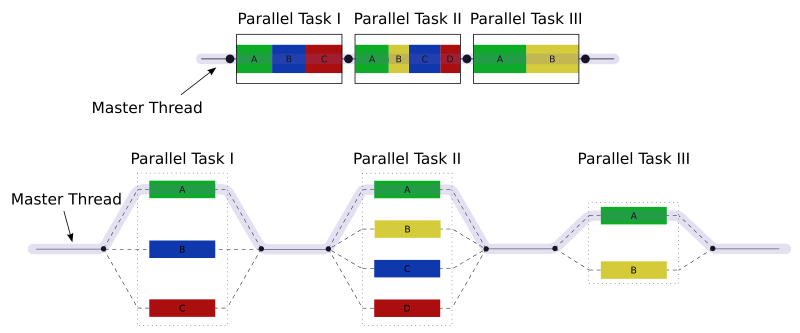
\includegraphics[width=4.8in,height=2in]{pic/3.png}
\caption{OpenMP原理}
\end{figure}

\item CUDA : Compute Unified Device Architecture(CUDA)是由英伟达公司创造的,用于GPU上的平行处理平台.利用CUDA,GPU不仅可以进行图形处理,还可进行其他的通用计算(所谓的GPGPU).

对于操作系统,它支持windows、linux、mac os三大主流系统.CUDA为开发者提供了虚拟指令集和并行计算单元的内存来进行运算.

\item TBB(Intel Threading Building Blocks):是一个由英特尔公司开发的C++模板库,主要目的是使得软件开发者更好的利用多核处理器.该库为开发者提供了一些线程安全的容器和算法,使得开发者无需过多关注系统线程的创建、同步、销毁等操作,将精力集中于业务逻辑的并行化,可以与OpenMP互为补充.
\end{enumerate}

\begin{table}[!hpb]
  \centering
  \begin{tabular}{|c|c|c|c|}
    \hline
    比较项目 & OpenMP & TBB & MPI \\ 
    \hline
    并行粒度 & 线程 & 线程 & 进程 \\
    内存模式 & 共享内存&共享内存&分布式内存\\
    适用环境 & 单机 & 单机 & 集群\\
    通讯机制&*&*&消息传递 \\
    易用性 & 高& 中 & 低 \\
    跨平台性 & 是&是&是\\
    并发数据结构 & 不支持 &支持&支持\\
    可扩展内存分配&不支持&支持&不支持\\
    \hline
  \end{tabular}
\caption{各种并行计算框架对比}
\end{table}

\subsubsection{想法来源及可能遇到的挑战}
并行计算如果按照硬件环境进行分类,那么以分布式计算为基础的计算机集群使其中典型的一类.以上三种并行框架大多是跨平台的,而inferno自身却具有分布式系统和以“资源皆文件”的优势,使得并行计算框架的构建更具有可执行性,但这个方向还鲜有相关研究.\n

根据相关调研,我们可能会面对下述问题 : 
\begin{enumerate}
\item 计算机集群实现分布式运算的特点,计算过程不一定是同步的,所以负载均衡是一个有挑战的问题,对应解决方案有Round-robin DNS,scheduling algorithms等.
\item 由于分布式计算需要共享实时数据,对于网络带宽以及低延迟网络的需求也是其需要考虑的问题,可以运用更高效率的传输媒介来处理.
\item 因为考虑的是并行框架,各个计算机、各个数据以及各个指令之间的竞争需要处理.例如:当计算机尝试覆盖相同或者旧的数据,而此时就的数据仍在被读取.结果可能是下面的一个或者多个情况:机器宕机、出现非法操作并结束程序、错误的读取旧数据、或者错误的写入新数据.在这里,竞争的危害出现于通过访问同一个信息通道的数据.解决的方法可以通过标记正在处理的数据以及标记读写来处理.   
\item 分布式系统中的另一个问题是容错性问题(fault-tolerance).这也是有名的拜占庭将军问题(Byzantine failures).在容错的分布式计算中,拜占庭失效可以是分布式系统中算法执行过程中的任意一个错误.这些错误被统称为“崩溃失效”和“发送与遗漏是失效”.当拜占庭失效发生时,系统可能会做出任何不可预料的反应.这些任意的失效可以粗略地分成以下几类;进行算法的另一步时失效,即崩溃失效:无法正确执行算法的一个步骤;执行了任意一个非算法指定的步骤.具体来说就是所写的并行框架在没有容错处理时出现让人匪夷所思的随机错误.具体可以通过口头消息算法或签名消息算法解决.
\end{enumerate}

\end{document}

%%% Local Variables:
%%% mode: latex
%%% TeX-master: t
%%% End: